%%%%%%%%%%%%%%%%%%%%%%%%%%%%%%%%%%%%%%%%%%%%%%%%%%%%%%%%%%%%%%%%%%%%%%%%%%
%%%%%                        Intro Générale                         %%%%%%
%%%%%%%%%%%%%%%%%%%%%%%%%%%%%%%%%%%%%%%%%%%%%%%%%%%%%%%%%%%%%%%%%%%%%%%%%%
%\phantomsection 
%\addcontentsline{toc}{chapter}{Introduction}
%\addtocontents{toc}{\protect\addvspace{10pt}}

%\vspace*{-1cm}
%\begin{flushright}
%\section*{\fontsize{20pt}{20pt}\selectfont\textnormal{Introduction}}
\chapter{Introduction}
\label{ch:intro}
%\end{flushright}
%\vspace{2cm}

\lhead[\fancyplain{}{Introduction}]
      {\fancyplain{}{}}
\chead[\fancyplain{}{}]
      {\fancyplain{}{}}
\rhead[\fancyplain{}{}]
      {\fancyplain{}{Introduction}}
\lfoot[\fancyplain{}{}]%
      {\fancyplain{}{}}
\cfoot[\fancyplain{}{\thepage}]
      {\fancyplain{}{\thepage}}
\rfoot[\fancyplain{}{}]%
     {\fancyplain{}{\scriptsize}}
     

%%%%%%%%%%%%%%%%%%%%%%%%%%%%%%%%%%%%%%%%%%%%%%%%%%%%%%%%%%%%%%%%%%%%%%%%%%
%%%%%                      Start part here                          %%%%%%
%%%%%%%%%%%%%%%%%%%%%%%%%%%%%%%%%%%%%%%%%%%%%%%%%%%%%%%%%%%%%%%%%%%%%%%%%%

\minitoc
\newpage

Hyperspectral (HS) imaging, also referred to as image spectrometry, stands as a significant advancement within geoscience and remote sensing (RS) owing to its ability to precisely identify a broad range of materials thanks to their spectral fingerprints.
In the past decade, substantial efforts have been directed towards the processing and analysis of HS data, predominantly under the guidance of domain experts.
Nevertheless, as the quantity of data continues to grow, new challenges arise to alleviate expensive and tedious manual labor, in order to enhance productivity.
Consequently, there is a pressing need for the development of more efficient and automated methods to address diverse applications of HS RS.
Examples of such tasks include large-scale land cover mapping, HS image restoration, HS unmixing, data fusion and multimodal data analysis.

Boosted by the recent advances in deep learning for computer vision, earth observation (EO) has witnessed a surge of deep models aiming to improve prediction performance over classical model-based image processing methods.
While the latter techniques have proven effective under highly idealized assumptions, their limited modeling capability often fail to grasp intricate real-world scenarios due to the existence of unknown, uncertain and unpredictable factors.
On the other hand, deep learning models benefit from extensive modeling capacity enabling them to handle considerably more complex scenes at the cost of potential overfitting.
That being said, the effectiveness of deep models primarily hinges on their ability to leverage prior knowledge through advanced network architecture design, empirical training techniques and huge amounts of annotated data.
Moreover, deep networks tend to lack \emph{interpretability}, a desirable property of learning models for scientific applications, due to their ``black box" nature.
Ideally, a reliable prediction model should not only perform accurately but also be able to explain its predictions.
To address this limitation, the field of explainable artificial intelligence (AI) has emerged as a burgeoning area of research.

Concurrently, at the crossroad between model-based methods and deep learning stands the emerging field of \emph{model-based deep learning}~\cite{shlezinger_model-based_2023} whose aim is to combine the advantages of both approaches, by embedding principled mathematical models within data-driven systems.
These hybrid approaches are generally task-specific, yet they may be relevant to a multitude of research domains provided that one has access to some level of reliable mathematical modeling.
One of the key strategies within model-based deep learning that we will delve into is \emph{algorithm unrolling} or \emph{deep unfolding}~\cite{monga_algorithm_2021}, aiming to transform iterative optimizers into trainable parameterized architectures.

Unrolling methods were first proposed to develop fast neural network approximations for sparse coding~\cite{gregor_learning_2010}.
The core concept revolves around training a non-linear, feed-forward predictor with a specific architecture and a fixed depth to produce the best possible approximation of the sparse code.
Unrolling methods have gained substantial popularity owing to their capacity to craft efficient, high-performance, and interpretable network architectures, all achieved with reasonably sized training datasets.

In this thesis, we present our contributions aligned with the aforementioned research directions, with a particular emphasis on their applications in HS imaging.
Building upon recent advancements in the restoration of natural images, we introduce a novel trainable two-layered spectral-spatial sparse coding model to tackle HS denoising.
We then shift our focus to blind HS unmixing, offering an efficient solution for an archetypal analysis formulation within a pure model-based framework.
Inspired by the interpretability and flexibility provided by the archetypal analysis formulation, we develop a new mixing model tailored for semi-supervised HS unmixing, addressing library mismatch.
Finally, we provide a comprehensive overview of image processing and machine learning techniques for HS unmixing, complemented by a Python package designed to facilitate the reproducibility of research findings in the field of unmixing.
For a deeper dive into these contributions, please refer to Section~\ref{sec:contrib}.
The remaining sections of this chapter offer an essential groundwork for the upcoming chapters.
First, we provide some background on HS imaging in Section~\ref{sec:HS}.
Next, we delve into the realm of HS restoration in Section~\ref{sec:denoising}.
Lastly, in Section~\ref{sec:unmixing}, we introduce the fundamental components of HS unmixing.

% Add the following sentences to the first contribution
%Beyond mere quantitative outcomes, we believe that our work sheds light on the efficiency of our models in learning a relatively concise set of parameters, while achieving state-of-the-art results.
%This efficiency is especially critical due to the limited availability of training data for HSI denoising and the challenges associated with training deep learning models for this purpose.
%Additionally, our study highlights the value of interpretable architectures, showcasing their adaptability to tackle broader issues such as blind denoising - a crucial aspect in the processing of HS images. 



% Perhaps remove this section
%Learning from data fundamentally requires a degree of \emph{simplicity}, often referred to as the \emph{inductive bias}, within the learning algorithm.
%The objective here is to incorporate and exploit some prior knowledge regarding the specific problem being addressed.
%As mentioned earlier, the choice of architecture is the primary form of inductive bias in deep neural networks.
%Another illustrative example of this is \emph{sparsity}, which guides the final model to only rely on a few relevant variables out of many available ones.

\section{Contributions of the thesis}
\label{sec:contrib}

This thesis makes significant contributions to the field of HS image processing, with a particular emphasis on the creation of data and computationally efficient methodologies.
Each of these contributions has resulted in the development of a corresponding open-source software package.
These contributions are presented hereafter.

\begin{itemize}
    \item Chapter~\ref{ch:T3SC} introduces a new trainable network architecture, called T3SC, derived from a sparse coding model tailored to address the specificity of HS images in the context of denoising.
    We extend the approach developed by~\cite{lecouat_fully_2020} for natural images restoration by adopting a two-layer model as a mean to provide a shared architecture for different HS sensors.
    Beyond mere quantitative outcomes, we believe that our work sheds light on the efficiency of our models in learning a relatively concise set of parameters, while achieving state-of-the-art results.
    This efficiency is especially critical due to the limited availability of training data for HS denoising and the challenges associated with training deep learning models for this purpose.
    Additionally, our study highlights the value of interpretable architectures, showcasing their adaptability to tackle broader issues such as blind denoising - a crucial aspect in the processing of HS images. 

    \begin{tcolorbox}[colback=gray!5!white,colframe=gray!75!black]
        T. Bodrito$^{*}$, A. Zouaoui$^{*}$, J. Chanussot, and J. Mairal. A trainable spectral-spatial sparse coding model for hyperspectral image restoration. In \emph{Advances in Neural Information Processing Systems (NeurIPS)}, 2021

        \vspace{1em}

        ($^{*}$equal contributions)
    \end{tcolorbox}

    \item In Chapter~\ref{ch:EDAA}, our attention turns to another critical task inherent to HS image processing: spectral unmixing. 
    We introduce a novel algorithm based on archetypal analysis for blind hyperspectral unmixing. 
    Our approach, called EDAA, leverages an entropic gradient descent strategy, steering the optimization process within the geometry induced by the negative entropy function.
    This framework is tailored to accommodate the constraints imposed by the linear mixing model.
    Notably, thanks to an efficient GPU-compatible implementation, we propose a model selection procedure that enhances the robustness of our method to hyper-parameter choices, all the while maintaining reasonable computational complexity.
    Finally, our work highlights the effectiveness of the archetypal analysis formulation as a viable approach to tackle blind HS unmixing.
    
    \begin{tcolorbox}[colback=gray!5!white,colframe=gray!75!black]
        A. Zouaoui, G. Muhawenayo, B. Rasti, J. Chanussot, and J. Mairal. Entropic descent archetypal analysis for blind hyperspectral unmixing. In \emph{IEEE Transactions on Image Processing}, 2023
    \end{tcolorbox}


    \item Chapter~\ref{ch:SUnAA} further exploits archetypal analysis in the context of semi-supervised HS unmixing.
    Our novel formulation, called SUnAA, assumes that the materials of interest, or \emph{endmembers}, are a convex combination of endmembers provided by a spectral library, with the added knowledge that the number of endmembers in the scene is known.
    Unlike most conventional sparse unmixing methods, the objective function in this formulation is non-convex.
    As a result, we employ an iterative approach to minimize this objective, leveraging the active set algorithm proposed in~\cite{chen_fast_2014}.

    \begin{tcolorbox}[colback=gray!5!white,colframe=gray!75!black]
        B. Rasti$^{*}$, A. Zouaoui$^{*}$, J. Mairal, and J. Chanussot. SUnAA: Sparse Unmixing using Archetypal Analysis. In \emph{IEEE Geosciences and Remote Sensing Letters}, 2023

        \vspace{1em}

        ($^{*}$equal contributions)
    \end{tcolorbox}


    \item Chapter~\ref{ch:HySUPP} serves as a comprehensive overview of both advanced and conventional unmixing approaches.
    We offer a critical comparison between advanced and conventional techniques depending on the level of prior knowledge available about the endmembers.
    We thoroughly assess the performance of various unmixing techniques using a diverse set of unmixing datasets, encompassing both simulated and real-world examples.
    Notably, we highlight the advantages of the three main unmixing categories - supervised, semi-supervised, and blind - in different unmixing scenarios.
    Finally, we provide an open-source Python package, named HySUPP, that contains an exhaustive list of unmixing methods, in order to foster research results reproducibility.

    \begin{tcolorbox}[colback=gray!5!white,colframe=gray!75!black]
        B. Rasti, A. Zouaoui, J. Mairal and J. Chanussot. Image Processing and Machine Learning for Hyperspectral Unmixing: An Overview and the HySUPP Python Package. \emph{arXiv preprint arXiv:2308.09375}, 2023
    \end{tcolorbox}
    
\end{itemize}


\section{Background on Hyperspectral Imaging}
\label{sec:HS}

% Add date?
Hyperspectral (HS) imaging consists of measuring the electromagnetic spectrum at each pixel location within a scene by using multiple contiguous spectral bands.
Thanks to its richer spectral information compared to traditional RGB images, HS imaging enables more precise materials identification.
This capability has led to a diverse array of applications in fields such as astronomy, agriculture, biomedical imaging and geosciences.
However, this technology also presents numerous challenges.
As a relatively new analytical technique, the potential of HS imaging has not yet been fully realized. 

\subsection{Characteristics}

HS imaging falls within the broader category of techniques commonly known as spectral imaging.
The term ``hyperspectral" has gained prominence over its counterpart, ``spectroscopy".
NASA played a pivotal role in developing this technology in the mid-1980s.
HS imaging is closely related to multispectral (MS) imaging.
HS imaging uses continuous and contiguous wavelength ranges (e.g., 400 to 1000 nm in 5 nm intervals), while MS imaging focuses on specific, selected wavelengths at discrete locations (e.g., 400-425, 550-570, 760-790, and 990-1010 nm, resulting in a four-band MS image).

In this thesis, we develop methods specifically tailored to HS imaging, drawing inspiration from various research domains, including computer vision, machine learning and signal processing.

\subsection{Acquisition}

HS sensors acquire data in the form of a series of images, with each image corresponding to a specific narrow wavelength range within the electromagnetic spectrum, often referred to as a spectral band.
These individual images are combined to construct a three-dimensional HS datacube ($x, y, \lambda$) for subsequent analysis.
In this context, $x$ and $y$ denote the two spatial dimensions of the scene, while $\lambda$ represents the spectral dimension.

There are four main techniques for acquiring the three-dimensional dataset of a HS cube.
The choice of technique ultimately depends on the specific application, given that each technique has context-dependent advantages and drawbacks.

% NOTE: Do I use the figure from Wikipedia?

\begin{itemize}
    \item \textbf{Spatial scanning}: Each two-dimensional sensor output represents a full slit spectrum ($x, \lambda$).
    A push broom scanner is commonly used to obtain slit spectra by projecting a strip of the scene onto a slit and dispersing the slit image with a prism or a grating.
    To ensure accurate image reconstruction, this technique requires stable mounts or precise pointing information.
    It finds practical applications in remote sensing (RS) and scanning materials in motion on a conveyor belt.
% Add stripe pattern
    
    \item \textbf{Spectral scanning}: Each two-dimensional sensor output represents a monochromatic map of the scene ($x, y$).
    Optical band-pass filters are commonly used to capture the scene by cycling through one after another while the platform remains stationary.
    However, it is important to note that spectral smearing can occur when objects within the scene are not stationary.
    While these sensors can be deployed on aircraft, it is often necessary to employ techniques that extract spatial features from each monochromatic image to realign the pixels and correct for any misalignment caused by the movement of the platform.
    
    \item \textbf{Snapshot}: HS devices designed for snapshot or non-scanning operations provide the complete datacube in a single capture, without the need for scanning.
    In this approach, a single snapshot captures a perspective projection of the entire datacube, from which its three-dimensional structure can be subsequently reconstructed.
    While various systems have been developed with a focus on increased light throughput and reduced acquisition time, it is worth noting that this approach often entails high computational demands and manufacturing costs.

    \item \textbf{Spatiospectral scanning}: Each two-dimensional sensor output represents a wavelength-coded spatial ($x, y$) map of the scene (i.e. with $\lambda = \lambda(y)$).
    This method uses a camera at some non-zero distance behind a basic slit spectroscope.
    Spatiospectral scanning combines some of the benefits of both spatial and spectral scanning techniques, effectively mitigating some of the drawbacks associated with each approach.
    
\end{itemize}

In this thesis, our techniques are designed to operate seamlessly across various acquisition modes, as they directly process the HS datacube.
However, in the section dedicated to image restoration, we concentrate on addressing a specific issue, namely, \emph{stripe} noise.
These artifacts commonly arise from defective spatial scanners.


\subsection{Applications}

Hyperspectral remote sensing (HS RS) finds diverse applications across numerous fields.
Initially designed for mining and geology, its utility has since expanded into a wide range of areas, including ecology, waste sorting, and historical manuscript research.
The accessibility of this technology to the public has grown steadily.
Leading organizations like NASA and USGS have compiled catalogs containing spectral signatures of various minerals and made them easily accessible to researchers through online repositories.
In what follows, we provide a brief overview of some significant applications of HS imaging.

\begin{itemize}
    \item \textbf{Agriculture}: HS imaging serves as a valuable tool for a variety of agricultural applications.
    It can be employed to identify different plant species and establish early warning systems for disease outbreaks.
    Furthermore, research efforts are focused on utilizing HS imaging to detect the chemical composition of plants, facilitating the monitoring of nutrient and water levels in irrigated wheat systems.
    HS cameras also offer the capability to identify stress caused by heavy metal accumulation in plants, providing an earlier and faster alternative to traditional post-harvest wet chemical methods.
    
    \item \textbf{Astronomy}: HS imaging plays a crucial role in astronomy, enabling the acquisition of spatially-resolved spectral images.
    Given the significance of spectral data as a diagnostic tool, the ability to obtain a spectrum for each pixel enhances the range of scientific inquiries that can be addressed in this field.
    % TODO more examples
    
    \item \textbf{Ecology}: The imperative to monitor greenhouse gas emissions from various industrial sources, including coal and oil-fired power plants and landfills, has become increasingly critical in recent times.
    By leveraging the distinctive spectral signatures of methane ($\text{CH}_4$), researchers can compile a comprehensive list of the largest emitters on a global scale, facilitated by satellite-based monitoring systems with worldwide coverage.
    
    \item \textbf{Food processing}: In the food processing industry, the synergy of HS imaging with advanced software empowers digital sorters to detect and eliminate defects and foreign materials that would otherwise remain unseen by conventional camera and laser sorting systems.
    A key advantage of this approach is its non-destructive nature.
    Consequently, this technology holds the potential to address a multitude of persistent product quality issues, offering a promising solution for the industry.
    
    \item \textbf{Historical studies}: The Archimedes Palimpsest is a significant parchment codex that holds two invaluable works by Archimedes (the \emph{Ostomachion} and the \emph{Method of Mechanical Theorems}), which were previously believed to have been lost.
    It also contains the sole surviving original Greek edition of his work, \emph{On Floating Bodies}.
    In the Middle Age, the manuscript was overwritten with a religious text.
    Shortly before its latest acquisition in 1998, counterfeit images were painted over portions of the text, obscuring their content.
    However, by analyzing 12-band multispectral (MS) images, researchers were able to unveil the concealed texts underneath the forged pictures, as well as decipher previously unreadable portions of the manuscript.
    
    
    \item \textbf{Waste sorting and recycling}: HS imaging plays a pivotal role in waste sorting and recycling by offering insights into the chemical composition of materials. 
    This capability proves invaluable in distinguishing between various substances with different fabric compositions, including the identification of natural, animal, and synthetic fibers.
    HS cameras can seamlessly integrate with computer vision systems, enabling the automated separation of plastic waste products and packaging by distinguishing between different types of plastics.
    
\end{itemize}

In this thesis, we do not focus on a specific application.
Rather, we tackle research problems, namely image restoration and spectral unmixing, that are fundamental and pervasive across all applications within the realm of HS imaging.

\subsection{Challenges}

The primary drawbacks of HS imaging revolve around cost and complexity.
To effectively analyze HS data, it requires powerful computing resources, sensitive detectors, and substantial data storage capabilities.
The data storage requirement is especially notable because uncompressed HS cubes constitute large, multidimensional datasets, often exceeding hundreds of megabytes in size.
These factors collectively contribute to the elevated costs associated with acquiring and processing HS data.
Furthermore, researchers are confronted with the challenge of programming HS satellites to autonomously sift through data and transmit only the most critical images.
This is essential, as the transmission and storage of such voluminous data can prove to be both technically challenging and financially burdensome.

In recent years, a multitude of HS RS missions have been launched with the aim of advancing our comprehension of Earth and its environment.
As the availability of RS data continues to expand, originating from satellite and airborne sensors on both large and global scales, traditional data processing and analysis tools have encountered limitations, unable to keep pace with the demands of the big data era.
Consequently, data-driven signal and image processing, along with machine learning (ML) models, have drawn increasing attention among researchers within the RS community.

HS imaging often faces limitations in either spectral or spatial resolution.
Moreover, a multitude of factors, including physical and chemical atmospheric effects, environmental conditions (e.g., soil interference, fluctuations in illumination, unpredictable shadows cast by clouds or buildings, variations in topography, and intricate noise patterns), have historically hindered traditional RS techniques, leading to predominantly qualitative analysis.
However, this paradigm has shifted in recent times with the emergence of non-convex optimization techniques, such as deep learning.
These advanced approaches have demonstrated their capability to effectively address increasingly complex scenarios.
Nonetheless, a significant drawback consists in the inherent lack of interpretability coming from these deep networks, which has emerged as a major concern for decision-makers.

Hence, there is a pressing need to develop techniques that are not only efficient but also interpretable, tailored to address the diverse spectrum of research problems specific to HS imaging.
This thesis focuses on two fundamental tasks related to HS data: image restoration and spectral unmixing.
These tasks are presented in the following sections, accompanied by a comprehensive list of related works.


\section{Image Restoration}
\label{sec:denoising}

Hyperspectral (HS) signals contain a wealth of information compared to RGB images.
However, this advantage comes with the challenge of managing intricate degradations originating from multiple sources, including sparse noise patterns like stripes, as well as photon and thermal noise~\cite{kerekes_hyperspectral_2003, rasti_noise_2018}.
Consequently, HS image denoising serves as a pivotal pre-processing step to increase image quality, facilitating subsequent tasks such as semantic segmentation and spectral unmixing.

Another substantial challenge arises from the scarcity of extensive, high-quality ground-truth datasets and the sheer diversity of sensor types employed in HS imaging.
This complexity poses significant hurdles in training ML models, such as convolutional neural networks (CNNs), for restoration tasks.

To navigate the scarcity of ground-truth data, the most successful approaches typically incorporate robust prior knowledge directly into the model architecture.
This prior knowledge may manifest as low-rank representations of input patches~\cite{fan_spatialspectral_2018, gong_low-rank_2020, rasti_automatic_2017, wang_hyperspectral_2021, zhao_hyperspectral_2015}, sparse coding techniques~\cite{dabov_image_2007, fu_adaptive_2015, gong_low-rank_2020}, or leveraging image self-similarities~\cite{maggioni_nonlocal_2013, peng_decomposable_2014, zhuang_hyperspectral_2017}.
These strategies have proven successful in the realm of RGB image processing~\cite{buades_non-local_2005} and are adapted to address the unique challenges posed by HS data.

We are now in shape to delve into the multitude of approaches employed for restoring HS data.
Our journey begins with an examination of model-based techniques, followed by an introduction to data-driven methods.
Subsequently, we will explore hybrid approaches and eventually focus on the more specific algorithm unrolling techniques.

\subsection{Model-based approaches}

Classical signal processing models for grayscale image denoising such as BM3D~\cite{dabov_image_2007}  may be
applied independently to each spectral band of HS signals. 
Not surprisingly, such an approach fails to capture relations between different channels and multi-band techniques have been shown to perform better. 
An extension of BM3D to volumetric data is proposed with BM4D~\cite{maggioni_nonlocal_2013}, which is more relevant for HS imaging.
GLF~\cite{zhuang_hyperspectral_2017} builds upon the same
principles as BM3D -- namely, exploiting self-similarities by grouping 3D
patches and collaborative filtering -- while introducing subspace
identification and data-adaptive filtering based on principal component
analysis.
GLF appears to be a very strong baseline, but is unfortunately very computationally demanding at test time.
Tensor-based methods such as LLRT~\cite{chang_hyper-laplacian_2017} are able to exploit the underlying low-rank structure of HS signals~\cite{fan_spatialspectral_2018, rasti_automatic_2017, zhang_hyperspectral_2014} and have shown particularly effective when combined with a non-local image prior as in NGMeet~\cite{he_non-local_2020}.
Finally, other approaches adapt traditional image processing priors such as
total variation~\cite{yuan_hyperspectral_2014, wang_hyperspectral_2021},
or wavelet sparsity \cite{othman_noise_2006, rasti_hyperspectral_2014}
to HS denoising, but they tend to perform worse than GLF, LLRT, or NGMeet, see~\cite{kong_comprehensive_2020} for a survey on denoising techniques for HS imaging.


\subsection{Data-driven approaches}

\subsubsection{Sparse coding and dictionary learning}

Dictionary learning~\cite{olshausen_emergence_1996} is an unsupervised learning technique consisting of representing a signal as a linear combination of a few elements from a learned dictionary, which has shown to be very effective for various image restoration tasks~\cite{elad_image_2006, mairal_sparse_2007}.
Several approaches have then combined dictionary learning and low-rank regularization.
For instance, 3D patches are represented as tensors in~\cite{peng_decomposable_2014} and are encoded by using spatial-spectral dictionaries~\cite{tucker_mathematical_1966}.
In~\cite{zhao_hyperspectral_2015}, 2D patches are extracted from the band-vectorized representation of the 3D HS data and sparsely encoded on a dictionary, while encouraging low-rank representations with a trace norm penalty on the reconstructed image.
The low-rank constraint can also be enforced by designing the dictionary as the result of the matrix multiplication between spatial and spectral dictionaries learned by principal component analysis as in~\cite{fu_adaptive_2015}.
However, these methods typically compute sparse representations with an iterative optimization procedure, which may be computationally demanding at test time.

\subsubsection{Deep learning}

Like BM3D above, convolutional neural networks for grayscale image denoising (\emph{e.g.}, DnCNN \cite{zhang_beyond_2017}) may also be applied to each spectral band, which is of course sub-optimal.
Because deep neural networks have been highly successful for RGB images with often low computational inference cost, there have been many attempts to design deep neural networks dedicated to HS denoising.
For instance, to account for the large number of hyperspectral bands, several approaches based on CNNs are operating on sliding windows in the spectral domain,~\cite{maffei_single_2020, shi_hyperspectral_2021, yuan_hyperspectral_2019}, which allows training models on signals with different number of spectral bands, but the sliding window significantly increases the inference time.
More precisely, attention layers are used in~\cite{shi_hyperspectral_2021}, while more traditional CNNs are used in~\cite{maffei_single_2020}, possibly with residual connections~\cite{yuan_hyperspectral_2019}.
Recently, an approach based on recurrent architecture was proposed in~\cite{wei_3-d_2020} to process signals with an arbitrary number of bands, achieving impressive results for various denoising tasks.

\subsection{Hybrid approaches}

SMDS-Net~\cite{xiong_smds-net_2020} adopts a hybrid approach between sparse coding and deep learning models by adapting the RGB image restoration method of~\cite{lecouat_fully_2020} to HS images.
SMDS-Net first denoises the input image with non-local means~\cite{buades_non-local_2005}, then performs subspace projection in the spectral domain using HySime~\cite{bioucas-dias_hyperspectral_2008}, before sparsely encoding 3D patches (cubes) with a trainable version of Tensor-based ISTA~\cite{qi_tensr_2016}.
Although this method reduces considerably the number of parameters in comparison to vanilla deep learning models, the spectral sliding window approach lacks interpretability since the same denoising procedure is applied across different bands, which may not suffer from the same level of noise.

\subsection{Algorithm Unrolling}

Algorithm unrolling, or deep unfolding, has found applications in recent years across a broad spectrum of domains, with computational imaging, including hyperspectral imaging, standing out as a prominent area of interest.
Many computational imaging research problems revolve around solving inverse problems, where retrieving the original data or image from observed measurements can be highly complex.
Traditional approaches to tackle these inverse problems have often followed a model-based strategy.
Within this paradigm, various techniques have emerged, such as sparse coding and low-rank matrix pursuit, which aim to find parsimonious representations of the underlying data.
Model-based techniques often require iterative approaches due to the scarcity of closed-form solutions.
These iterative algorithms form a rich domain of research, providing a robust foundation and ample prospects for the application of algorithm unrolling techniques.

For instance, SMDS-Net~\cite{xiong_smds-net_2020} harnesses the power of algorithm unrolling, a technique initially introduced in the seminal work of \cite{gregor_learning_2010}.
The primary aim of algorithm unrolling is to establish a connection between iterative algorithms and neural network architectures.
Figure~\ref{fig:unrolling} offers a high-level visualization of this framework, wherein each iteration of the algorithm corresponds to a distinct layer within the network.
Concatenating these layers effectively constructs a deep neural network.
The process of passing data through this network is equivalent to executing the iterative algorithm for a finite number of iterations.
Furthermore, the algorithm's parameters, including model parameters and regularization coefficients, directly translate into network parameters.
Consequently, this network can be trained through backpropagation, leading to model parameters that are learned from real-world training datasets.
This trained network can be naturally perceived as a parameter-optimized algorithm, effectively addressing the interpretability limitations commonly encountered in conventional neural networks.

\begin{figure}[h]
	\centering
	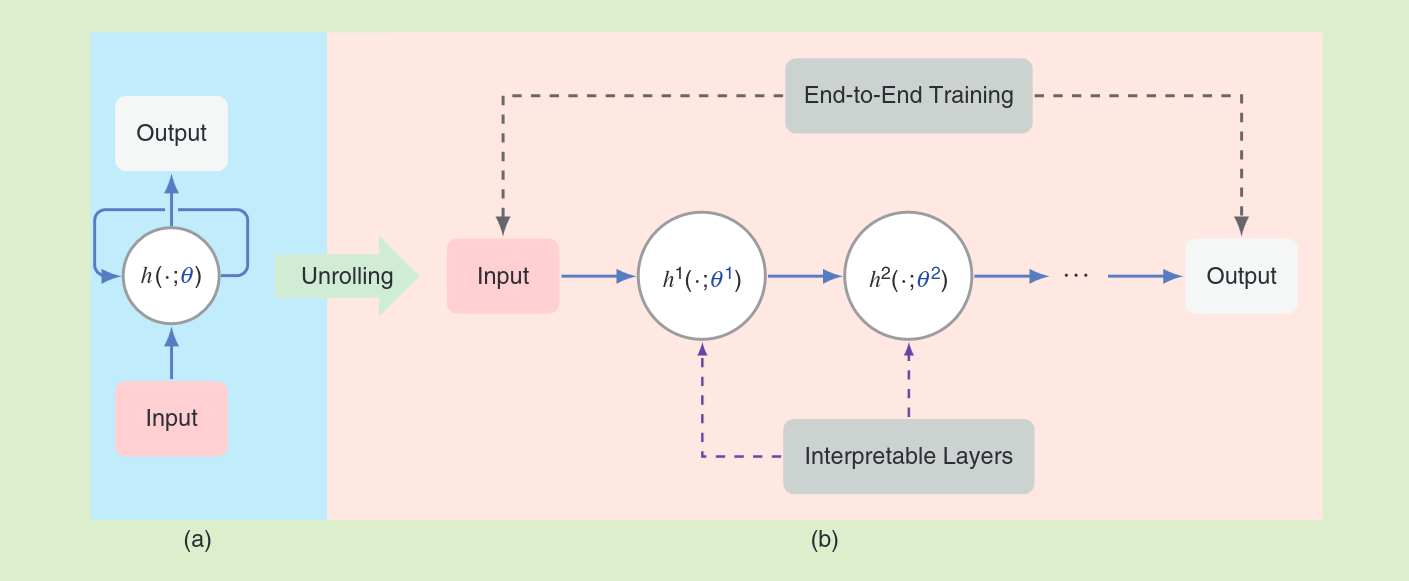
\includegraphics[width=\textwidth]{AlgorithmUnrolling.png}
	\caption{A high-level overview of algorithm unrolling from~\cite{monga_algorithm_2021}. 
 Given (a) an iterative algorithm, (b) a corresponding deep network can be generated by cascading the algorithm iterations $h$. 
 The iteration step $h$ in (a) is executed a number of times, resulting in the network layers $h^1, h^2, \ldots$ in (b). 
 Each iteration $h$ depends on algorithm parameters $\theta$, which are transferred into network parameters $\theta^1, \theta^2, \ldots$.
 Instead of determining these parameters through cross-validation and analytical derivations, $\theta^1, \theta^2, \ldots$ are learned from training data sets through end-to-end training.
 In this way, the resulting network can achieve better performance than the original iterative algorithm.
 In addition, the network layers naturally inherit interpretability from the iteration procedure.
 The learnable parameters are colored in blue.
 }
	\label{fig:unrolling}
\end{figure}

\subsubsection{LISTA for image denoising with dictionary learning}

We now focus on the Learned Iterative Shrinkage and Thresholding Algorithm (LISTA) applied to image denoising with dictionary learning.

% TODO paragraph Elad
A classical approach introduced by \cite{elad_image_2006} for image denoising consists in considering the set of small overlapping image patches (\emph{e.g.}, $8 \times 8$ pixels) from a noisy image, and compute a sparse approximation of these patches onto a learned dictionary.
The clean estimates for each patch are then recombined to produce the full image.

Formally, let us consider a noisy image $\yy \in \Real^{c \times h \times h}$ with $c$ channels and two spatial dimensions.
We denote by $\yy_1, \yy_2, \ldots, \yy_n$ the $n$ overlapping patches from $\yy$ of size $c \times s \times s$, which we represent as vectors in $\Real^{m}$ with $m = c s^2$.
Assuming that a dictionary $\D = \left[\dd_1, \ldots, \dd_p\right] \in \Real^{m \times p}$ is given -- we will discuss later how to obtain a ``good" dictionary -- each patch $\yy_i$ is processed by computing a sparse approximation:
\begin{equation}
\label{eq:SC}
    \min_{\alphab_i \in \Real^p} \frac{1}{2} \parallel \yy_i - \D \alphab_i \parallel_2^2 + \lambda \parallel \alphab_i \parallel_1,
\end{equation}
where $\parallel . \parallel_1$ is the $\ell_1$-norm, which is known to induce sparsity in the problem solution \cite{mairal_sparse_2014}, and $\alphab_i$ is the sparse code representing the patch $\yy_i$, while $\lambda > 0$ is a regularization parameter controlling sparsity.
Note that the $\ell_0$-penalty, which counts the number of non-zero elements, could also be used, leading to a combinatorial problem whose solution is typically approximated by a greedy algorithm.
After solving the $n$ problems (\ref{eq:SC}), each patch $\yy_i$ admits a ``clean" estimate $\D \alphab_i$.
Because each pixel belongs to several patches, the full restored image $\hat{\xx}$ is obtained by averaging these estimates.

Finding a good dictionary can be achieved in various manners.
In classical dictionary learning algorithms, $\D$ is optimized such that the sum of the loss functions (\ref{eq:SC}) is as small as possible, see \cite{mairal_sparse_2014} for a review.
Adapting the dictionary with supervision is also possible \cite{mairal_task-driven_2012}, as discussed next.


%The pursuit of efficiently representing signals has long been a central problem in signal processing, epitomized by the widely-studied sparse coding problem.
%Sparse coding involves finding a sparse representation of an input vector $\yy \in \Real^m$ using an overcomplete dictionary $\D \in \Real^{m \times p}$ (where $p > m$).
%In essence, it seeks a sparse code $\alphab \in \Real^p$ such that $\yy \approx \D \alphab$, while encouraging many coefficients in $\alphab$ to be zero or small in magnitude.
%One common approach to solving this problem is by minimizing the following convex optimization problem:


The proximal gradient descent method called Iterative Shrinkage and Thresholding Algorithm (ISTA)~\cite{figueiredo_em_2003, daubechies_iterative_2004} is a popular method for solving the optimization problem (\ref{eq:SC}) iteratively.
In its simplest form, ISTA performs the following iterations:
\begin{equation}
\label{eq:ISTA}
    \alphab_i^{(t+1)} = S_{\lambda}\left[\alphab_i^{(t)} + \eta \D^{\top}\left(\yy_i - \D \alphab_i^{(t)} \right)\right], \quad t=0,1,\ldots,
\end{equation}
where $\eta$ is a positive parameter controlling the iteration step size, and $S_{\lambda}(.)$ is the soft-thresholding operator defined elementwise as
\begin{equation}
\label{eq:soft-thresholding}
    S_{\lambda}(u) = \text{sign}(u) \cdot \max\left\{|u| - \lambda, 0\right\}.
\end{equation}

In essence, ISTA combines a gradient step of $\big|\big| \yy - \D \alphab \big|\big|_2^2$ with a projection onto the $\ell_1$ ball.

LISTA corresponds to an adaptation of ISTA by recasting its iteration into a single network layer.
This layer encompasses various analytic operations, including matrix-vector multiplication, summation, and soft-thresholding.
These operations are reminiscent of those found in a neural network.
Executing LISTA for $T$ iterations is akin to cascading $T$ such layers, effectively creating a $T$-layer deep network.

Within this unrolled network, various parameter substitutions can be made, such as introducing $\C \in \Real^{m \times p}$ and turning the scalar regularization parameter $\lambda$ into a vector $\lambdab \in \Real^p$ to effectively transform (\ref{eq:ISTA}) into
\begin{equation}
\label{eq:ISTA_C}
    \alphab_i^{(t+1)} = S_{\lambdab}\left[\alphab_i^{(t)} + \C^{\top}\left(\yy_i - \D \alphab_i^{(t)} \right)\right], \quad t=0,1,\ldots,
\end{equation}
as done in \cite{simon_rethinking_2019, lecouat_fully_2020}, where $S_{\lambdab}$ corresponds to the vectorized soft-thresholding operator defined in (\ref{eq:soft-thresholding}).
Lastly, another dictionary $\W$ is used to obtain a clean estimate $\W \alphab_i^{(T)}$ for each patch $\yy_i$, where $T$ is the number of LISTA steps.
The reason for allowing a different dictionary $\W$ than $\D$ is to correct the potential bias due to $\ell_1$-minimization.
These substitutions expand the representation power of the unrolled network and provide a more generalized parametrization compared to the original ISTA.

% TODO Clean this
Finally, the denoised image $\hat{\xx}$ is reconstructed by averaging the patch estimates:
\begin{equation}
\label{eq:reconstruction}
    \hat{\xx} = \frac{1}{m} \sum_{i=1}^n \R_i \W \alphab_i^{(T)},
\end{equation}
where $\R_i$ is the linear operator that places the patch $\hat{\xx_i}$ at position $i$ in the image, and we assume -- by neglecting border effects for simplicity -- that each pixel admits the same number $m$ of estimates.


The unrolled network's parameters, namely $\C$, $\D$, $\W$, and $\lambdab$, are optimized by training with a set of pairs of noisy/clean images in a supervised fashion.
We remark that the estimate $\hat{\xx}$ is obtained from a noisy image $\yy$ by a sequence of operations that are differentiable almost everywhere, as in typical neural networks with rectified linear unit activation functions, which allows the use of backpropagation to update the network's parameters.
A typical loss, which we optimize by stochastic gradient descent \cite{lecun_efficient_2002}, is then:
\begin{equation}
\label{eq:loss_LISTA}
    \min_{\C, \D, \W, \lambdab} \mathbb{E}_{\xx, \yy} \left[\parallel \hat{\xx}(\yy) - \xx \parallel^2\right],
\end{equation}
where $(\xx, \yy)$ is a pair of clean/noisy images drawn from some training distribution from which we can sample, and $\hat{\xx}(\yy)$ is the clean estimate obtain from (\ref{eq:reconstruction}), given the noisy image $\yy$.

It is worth noting that empirical evidence suggests that the number of layers $T$ in the trained LISTA can be significantly smaller than the number of iterations required for ISTA to converge to a solution that corresponds to a given input observation \cite{gregor_learning_2010}.

%\begin{figure}[h]
%	\centering
%	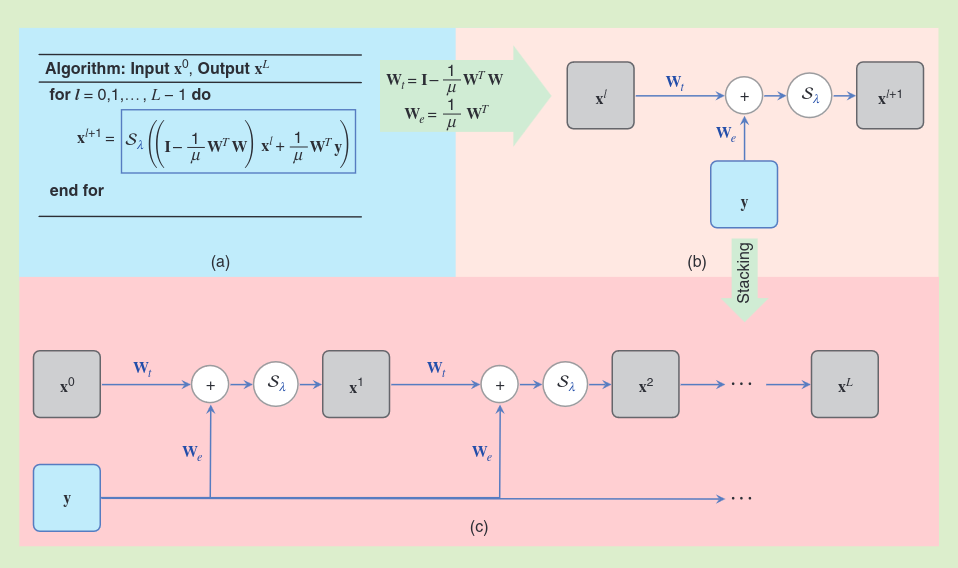
\includegraphics[width=\textwidth]{LISTA.png}
%	\caption{The LISTA from \cite{monga_algorithm_2021}. One iteration of the ISTA executes a linear operation and then a nonlinear one and thus can be recast into a network layer; by stacking the layers together, a deep network is formed. 
% The network is subsequently trained using paired inputs and outputs by backpropagation to optimize the parameters $\W_t$, $\W_e$, and $\lambda$; $\mu$ is a constant parameter that controls the step size of each iteration. 
% The trained network, a LISTA, is computationally more efficient compared with the original ISTA. 
% The trainable parameters in the network are colored in blue.
% In practice, $\W_t$, $\W_e$, and $\lambda$ may vary in each layer. (a) An ISTA. (b) A single network layer. (c) An unrolled deep network.}
%	\label{fig:LISTA}
%\end{figure}




\section{Spectral Unmixing}
\label{sec:unmixing}
Spectral unmixing is a crucial processing technique in hyperspectral (HS) remote sensing (RS).
The ability to separate and identify distinct materials within an image is made possible by the continuous spectra recorded by HS sensors.
Employing endmembers, which represent distinctive spectral signatures of macroscopic materials, unmixing algorithms can disentangle the blended spectral data into its individual components.
Nevertheless, the inherent challenges of low spatial resolution, multiple scattering, and intimate mixture typically yield measured spectra within a pixel that is a complex mixture of pure spectra from constituent materials, making unmixing a challenging task.
Figure~\ref{fig:unmixing} illustrates the spectral mixing occurring at the pixel level within a scene captured by a HS camera.

\begin{figure}[h]
	\centering
	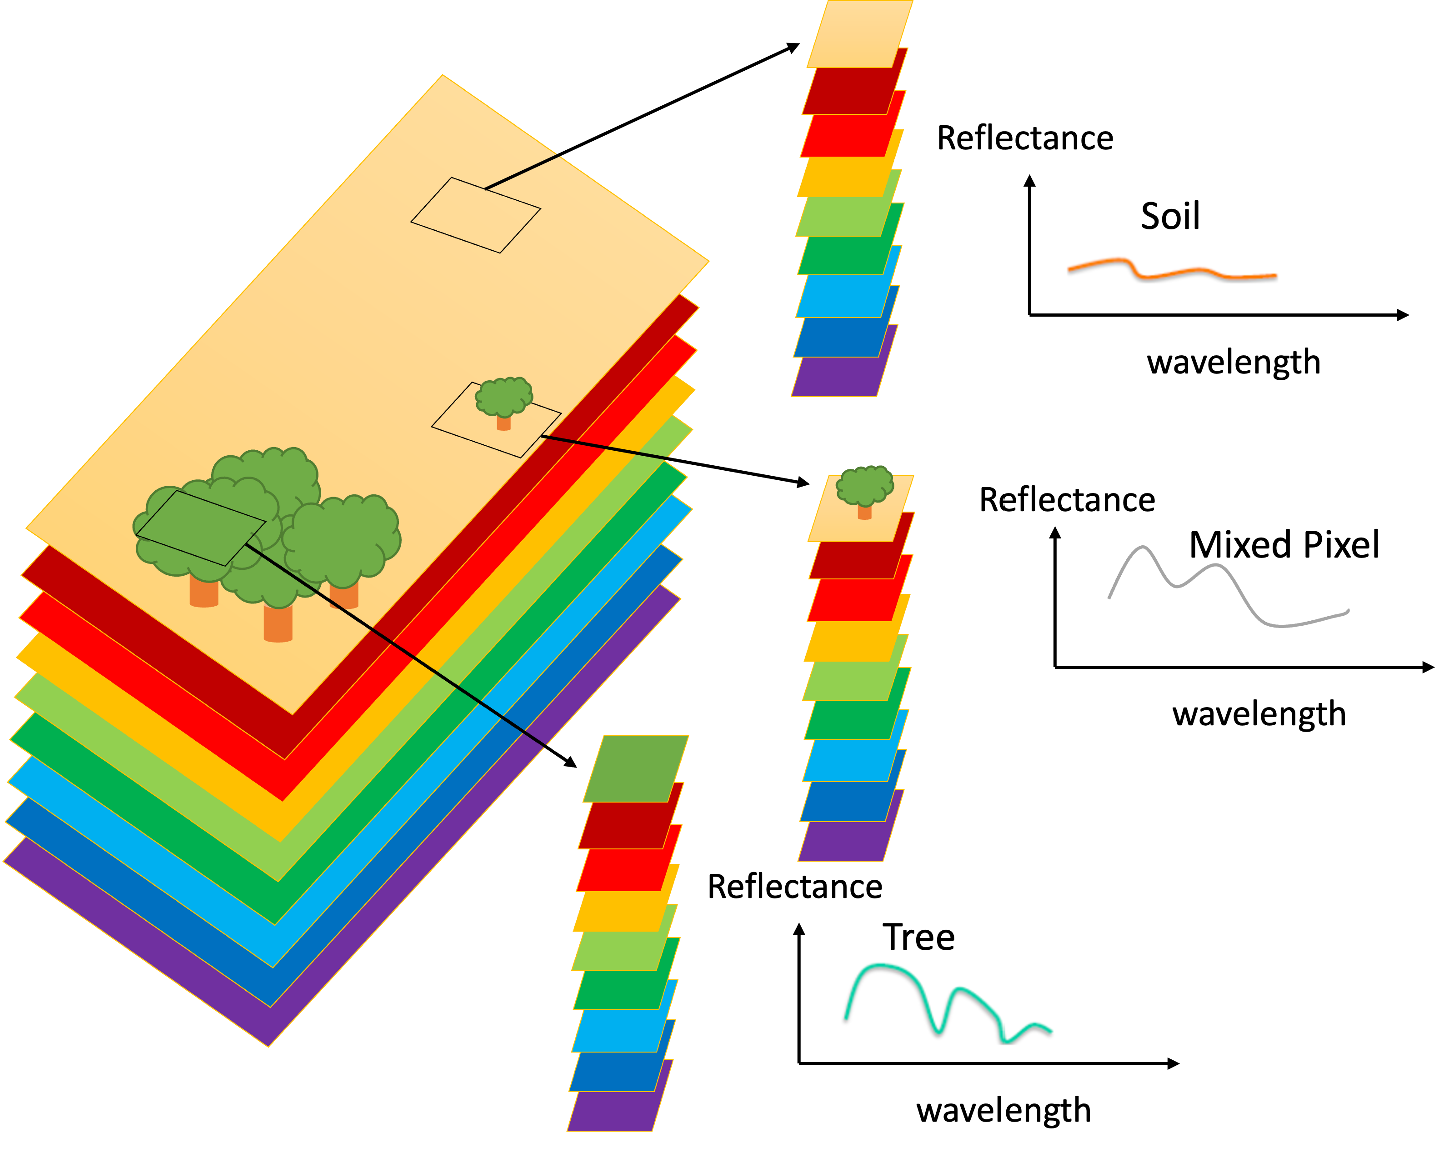
\includegraphics[width=0.6\textwidth]{fichiers_latex/Intro/Unmixing4.pdf}
	\caption{Illustration of pure and mixed pixels within an HS image from \cite{rasti_image_2023}. 
 In this context, each pixel comprises a spectrum generated by concatenating spectral bands, with each spectrum corresponding to reflectance at a specific wavelength.
 The top and bottom pixels are considered pure, as they consist of a single macroscopic material.
 In contrast, the middle pixel represents a mixture of tree and soil components.}
	\label{fig:unmixing}
\end{figure}

In the realm of HS RS, a mixing model serves as a representation of the observed spectral pixel, encapsulating the interplay between endmembers and their corresponding fractional abundances within the pixel's spatial domain.
Unmixing, in turn, involves the estimation of these fractional abundances.
This estimation can occur through various means, such as direct estimation or extraction of endmembers or reliance on a pre-existing library of endmembers.
Additionally, unmixing may encompass the determination of the number of endmembers present in the scene.
The nature of the mixing model can be either linear or nonlinear, depending on the interaction between incident light and the materials present within the scene or sample.
This thesis mainly focuses on the linear mixing model (LMM), whereby the endmembers are assumed to be linearly mixed.

In the subsequent sections, we will delve deeper into the underlying assumptions of the LMM.
We will then introduce various unmixing scenarios based on the level of prior knowledge available regarding the endmembers.
Following that, our focus will shift to archetypal analysis as a model formulation for linear unmixing.
Lastly, we will explore the different optimization strategies employed for conducting unmixing in HS imaging.

\subsection{Linear mixing model}


The LMM assumption holds true when each incident light ray interacts with a single material prior to reaching the HS sensor.
It is a common and valid assumption in Earth Observation (EO) applications, especially in macroscopic scenarios.
In these scenarios, the sensor's spatial resolution plays a pivotal role, as pixels may encompass multiple materials, leading to spectra that are mixtures of various substances.

Figure~\ref{fig:LU} provides a simplified illustration of the sensing process using a satellite equipped with a HS sensor.
The sensor records a pixel containing three distinct materials: water, tree, and soil.
At the sensor level, radiance is converted to reflectance, and atmospheric corrections are applied to compensate for atmospheric absorbance and light scattering effects.
This correction results in reflectance values ranging from zero to one.
Additionally, two physical constraints are imposed on the abundance fractions, namely the abundance non-negativity constraint (ANC) and the abundance sum-to-one constraint (ASC).

\begin{figure}[h]
	\centering
	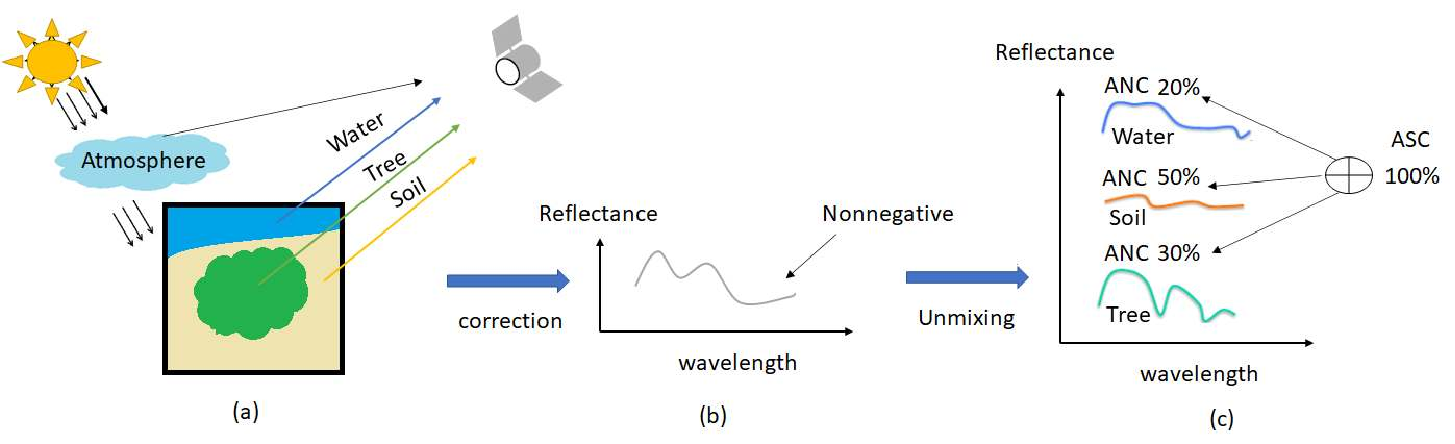
\includegraphics[width=\textwidth]{LUabs3.pdf}
	\caption{Illustration of the linear unmixing pipeline from \cite{rasti_image_2023}.
 (a) Sensing a mixed pixel; (b) Reflectance of the mixed pixel; (c) Schematic of linear unmixing.
        }
	\label{fig:LU}
\end{figure}

Formally, assuming the sensor records $p$ spectral bands, the LMM states that a $p$-dimensional pixel $\yy$ is represented as a linear combination of the endmembers within the pixel.
Let $\E = \left[\ee_1, \ldots, \ee_r \right] \in \Real^{p \times r}$ be a matrix containing $r$ endmembers, then:
\begin{equation}
    \label{eq:lmm}
    \yy = \E \abold + \nn, \quad \text{s.t.} \quad \sum_{i=1}^r \abold_i = 1, \; \abold_i \geq 0, \; i = 1, 2, \ldots, r,
\end{equation}
where $\abold$ is a $r$-dimensional vector corresponding to the abundance fractions associated to each endmembers, and $\nn$ is a $p$-dimensional random vector encompassing noise and model error.

Using matrix notations, we can represent the $n$ pixels by $\Y = \left[\yy_1, \ldots, \yy_n\right] \in \Real^{p \times n}$.
The LMM now writes as
\begin{equation}
    \label{eq:LMM}
    \Y = \E \A + \N, \quad \text{s.t.} \quad \A \geq 0, \; \1_r^{\top} \A = \1_n^{\top}, 
\end{equation}
where $\N \in \Real^{p \times n}$ denotes the noise and model error, $\A = \left[\abold_1, \ldots, \abold_n\right] \in \Real^{r \times n}$ is the abundance matrix containing the fractional abundances of each endmembers at every pixel, and $\1_d$ is a $d$-dimensional vector of ones.

In this configuration, the LMM assumes a known and fixed number of endmembers, denoted as $r$.
In this context, the LMM can be interpreted as a low-rank mixture model, where the rank corresponds to the number of endmembers.
Estimating the number of endmembers present in a scene is a challenging task that falls outside the scope of this thesis.
It is important to note that this information is not always required for unmixing.
Alternatively, one can consider the redundant linear mixture model, which can be expressed as:
\begin{equation}
    \label{eq:redundant}
    \Y = \D \X + \N \quad \text{s.t.} \quad \X \geq 0.
\end{equation}
Here $\D = \left[\dd_1, \ldots, \dd_m\right] \in \Real^{p \times m}$ represents a spectral library containing $m$ endmembers, and $\X = \left[\xx_1, \ldots, \xx_n\right] \in \Real^{m \times n}$ represents the unknown abundances to be estimated.
It is worth noting that the dictionary $\D$ is often overcomplete, meaning that $p < m$, and it should be well-designed to include the endmembers present in the scene.
When a well-designed dictionary is employed, $\X$ often exhibits sparsity properties because the pixels in the scene are usually composed of only a small number of dictionary elements, or atoms.

% TODO Mention challenges (number of endmembers)


\subsection{Unmixing scenarios}

Unmixing techniques can be categorized into three main groups based on the level of prior knowledge about endmembers.
Supervised and unsupervised (blind) approaches employ the low-rank mixing model. while semi-supervised unmixing relies on the redundant linear model.
It is important to clarify that the terminology used for these configurations should not be confused with the supervision setups commonly encountered in classical machine learning.
In this context, we exclusively refer to methods that do not have access to ground-truth abundances.
Therefore, all learning-based approaches are inherently unsupervised when it comes to learning.

Supervised unmixing assumes that a set of endmembers, denoted as $\E \in \Real^{p \times r}$, is known in advance, leaving only the task of estimating the abundances.
In contrast, blind unmixing aims to simultaneously estimate both endmembers and abundances without prior knowledge other than assuming the number of endmembers, $r$, to be known.
Semi-supervised unmixing leverages an existing library of endmembers, which should be sufficiently well-designed to include the materials present in the scene.
When the dictionary $\D \in \Real^{p \times m}$ is overcomplete ($p < m$), the goal in semi-supervised unmixing is often to achieve sparse estimates for the abundances, leading to its categorization as sparse unmixing.
Figure~\ref{fig:scenarios} provides an illustration of the three main types of unmixing.


\begin{figure}[h]
	\centering
	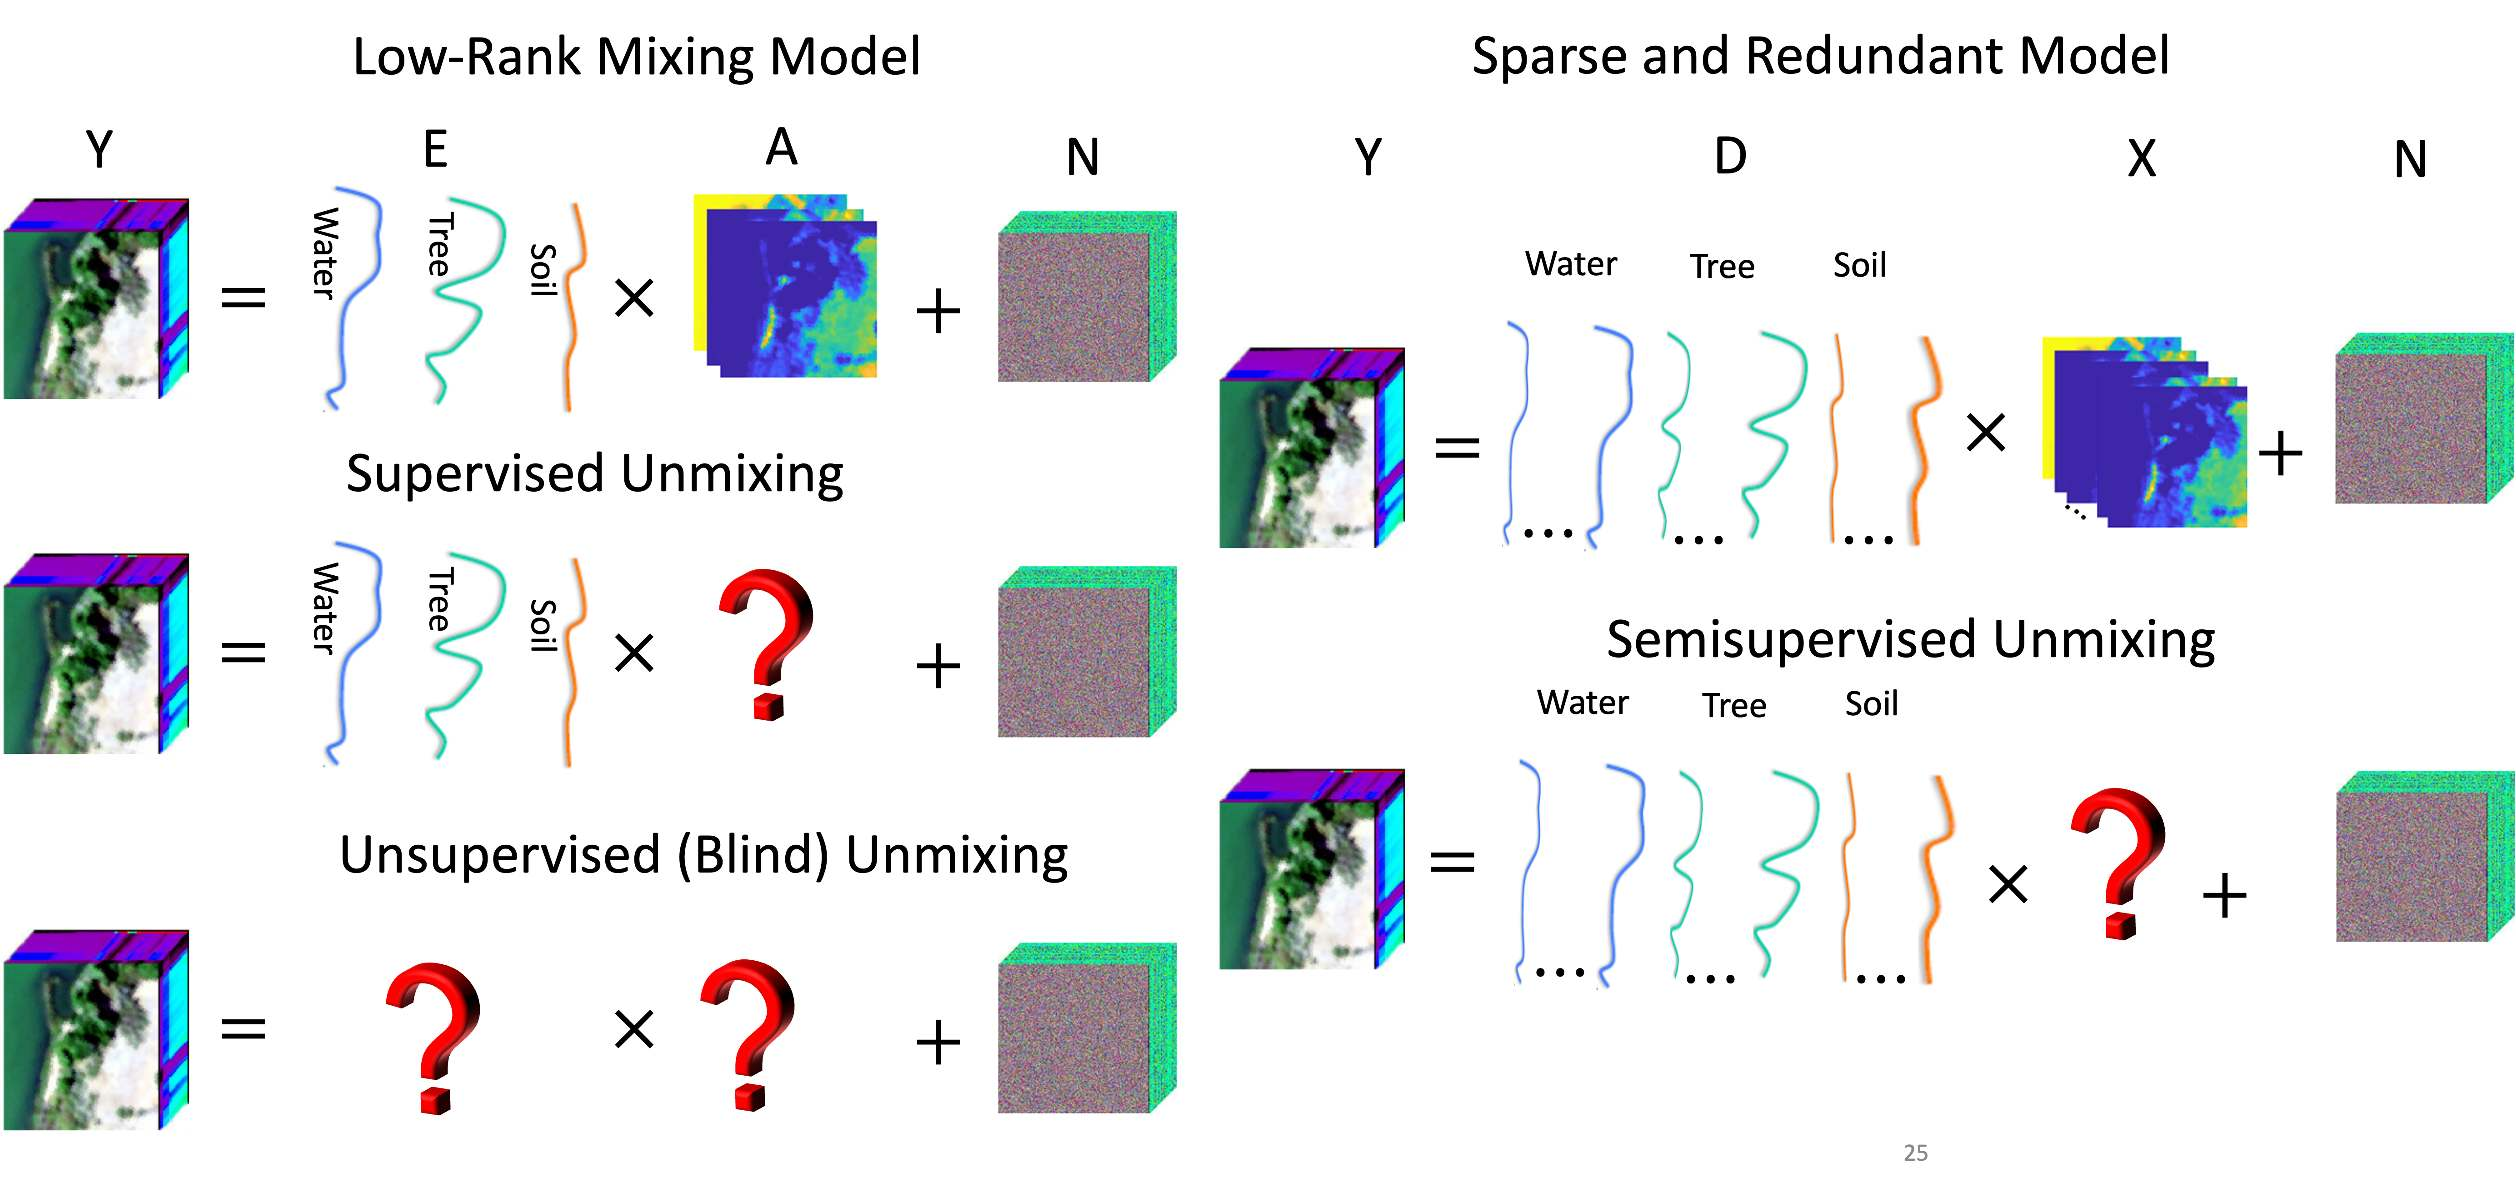
\includegraphics[width=\textwidth]{Models_LR_Sparse.pdf}
	\caption{Illustration of different types of linear unmixing from \cite{rasti_image_2023}.}
	\label{fig:scenarios}
\end{figure}

\subsubsection{Supervised unmixing}

In supervised unmixing, we assume that the endmembers are known, and the goal is to estimate the abundance matrix $\A \in \Real^{r \times n}$.
These endmembers can be obtained through various means, including field or laboratory measurements, selection from an existing spectral library, or direct extraction from the data.
However, selecting endmembers from a spectral library may not always yield optimal abundance estimations due to variations in the imaging setup.

Alternatively, endmembers can be directly extracted or estimated from the data points using geometrical approaches.
This extraction process can be challenging because the recorded data may not contain pure pixels, which are pixels containing a single macroscopic material, for all the materials present in the scene.
While many endmember extraction techniques are built on the assumption of having pure pixels, this assumption may not hold in practice.

It is important to note that we consider methods involving a sequential process of endmember extraction and subsequent abundance estimation to be categorized as supervised unmixing.
In general, abundance estimation does not affect endmember estimation due to the order in the processing chain.


\subsubsection{Blind unmixing}

In contrast, blind unmixing encompasses approaches that simultaneously estimate both endmembers and abundances.
This field of research comprises various paradigms and techniques.
It is worth noting that blind unmixing methods often face challenges related to their inherent non-convexity.
As a result, the optimization procedures used in these methods can be sensitive to initialization.
Therefore, it is common practice to initialize the endmember estimates using a geometrical endmember extraction approach to provide a starting point for the optimization process.

\subsubsection{Semi-supervised unmixing}

Finally, semi-supervised unmixing relies on the availability of an endmember library, making the selection or construction of this library a critical step in the process.
Blindly selecting a library without careful consideration and additional processing steps can lead to suboptimal results.
Two major paradigms are commonly used in semi-supervised unmixing: Multiple Endmember Spectral and Mixture Analysis (MESMA~\cite{roberts_mapping_1998}) and sparse unmixing.
MESMA was developed to address spectral variability by incorporating endmember variability into the library.
In this setup, the spectral library is designed to represent the variability of the endmembers present.
On the other hand, sparse unmixing, introduced in \cite{bioucas-dias_alternating_2010}, seeks a sparse solution based on the available library.
In both paradigms, the library must adequately represent the materials present in the scene, meaning it should contain all the endmembers present.
Various methods can be used to obtain such a library, including field or laboratory measurements, construction using observed data (often assuming the existence of pure pixels), and construction using physical models.

\subsection{Archetypal Analysis}

Now, we turn our attention to archetypal analysis (AA), a natural formulation for blind unmixing under the assumption of the LMM.
AA essentially represents endmembers as convex combinations of a few pixels found in the HS image.
In real HS data, pure pixels, which contain a single material and are essential for traditional endmember extraction techniques, are often missing due to various factors such as atmospheric conditions, changes in illumination, and environmental influences.
In the AA framework, not only are pixels viewed as linear combinations of estimated endmembers under the LMM, but the estimated endmembers themselves are modeled as convex combinations of pixels.
AA, initially introduced by Cutler and Breiman in 1994~\cite{cutler_archetypal_1994}, is a specific case of non-negative matrix factorization (NMF)~\cite{lee_algorithms_2000, paatero_positive_1994}, a popular approach for blind unmixing.
AA has the advantage to be more interpretable than NMF because the basis elements (\emph{i.e.}, endmembers) are directly constructed from the data points (\emph{i.e.}, pixels).
In addition, since the estimated endmembers generally correspond to averaging the contributions of several pixels, the resulting spectra appear more robust to noise and spectral variability than pure pixel methods that only rely on a single pixel per endmember.
However, AA usually suffers from a high data fitting error because the basis elements are constrained to be contained in the convex cone of the data points \cite{de_handschutter_near-convex_2019}.

\subsubsection{Non-negative matrix factorization}

Formally, within the LMM framework presented in (\ref{eq:LMM}), we investigate the blind unmixing scenario where both the mixing matrix, denoted as $\E$, and the abundance matrix, referred to as $\A$, are unknown.
The only prior knowledge assumed is the number of endmembers present in the scene, denoted as $r$.
As $\E$ represents the reflectance of the materials of interest across $p$ spectral channels, it is essential that its elements are non-negative, satisfying $\E \geq 0$.
Similarly, $\A$, which contains the abundances for each pixel in its columns, must also adhere to non-negativity constraints.
Furthermore, each column of $\A = \left[\abold_1, \ldots, \abold_n\right] \in \Real^{r \times n}$ should sum to one, ensuring that it forms a valid probability distribution.
This condition is equivalent to stating that each column of $\A$ belongs to the simplex $\Delta_r$, defined as:
\begin{equation}
    \label{eq:simplex}
    \Delta_r = \left\{\abold \in \Real^r \; \text{s.t.} \; \abold \geq 0 \; \text{and} \; \sum_{j=1}^{r} \abold[j] = 1\right\}.
\end{equation}

The LMM (\ref{eq:LMM}) yields the classical optimization problem
\begin{argmini}
  {\E,\A}{\frac{1}{2}\|\Y - \E \A\|_F^2,}{\label{eq:NMF}}{}
  \addConstraint{\E}{ \geq 0}
  \addConstraint{\abold_{i}}{\in \Delta_r \; \text{for} \; 1 \leq i \leq n},
\end{argmini}
which is a variant of NMF.
In essence, NMF involves decomposing a matrix representing the HS signal into the product of two matrices, both containing non-negative entries.
One matrix represents the endmembers, and the other represents the abundances for each pixel, typically with the constraint that the abundances sum to one.
Various NMF variants have been proposed for blind unmixing.

For instance, the Minimum Volume Constrained Non-Negative Matrix Factorization (MVC-NMF) method \cite{miao_endmember_2007} incorporates a minimum volume term for endmembers, eliminating the pure pixel assumption.
Minimum Dispersion Constraint NMF (MiniDisCo) \cite{huck_minimum_2010} introduces a regularization function known as dispersion to encourage endmembers with minimum variance, thus preventing degenerate solutions and enhancing unmixing robustness, particularly for flat spectra.
Another framework proposed in \cite{zhuang_regularization_2019} combines a data fidelity term with a minimum volume regularization term for endmembers, offering flexibility in the choice of regularization form. The authors also present an approach for automatic regularization parameter tuning.

Furthermore, various regularization functions have been designed for abundances in NMF, as seen in \cite{zymnis_hyperspectral_2007, yang_blind_2010, yao_nonconvex-sparsity_2019}.
It is important to note that standard NMF employs a least-squares objective function as in (\ref{eq:NMF}), which may not be optimal for handling noise and outliers in the data.
Consequently, alternative approaches like general loss-based NMF \cite{peng_general_2020} and self-paced NMF \cite{peng_self-paced_2021} have been proposed.
These methods employ different optimization criteria that can enhance robustness when dealing with noisy data and outliers.

\subsubsection{Modeling assumptions}

The AA formulation we consider introduces a constraint that enforces endmembers to be expressed as convex combinations of the pixels within the HS image $\Y$.
In other words, there exists a matrix $\B = \left[\bb_1, \ldots, \bb_r\right] \in \Real^{n \times r}$ such that $\E = \Y \B$, and the columns of $\B$ are constrained to lie within the simplex $\Delta_n$.
This results in the following optimization problem:

\begin{argmini}
  {\B,\A}{\frac{1}{2}\|\Y - \Y \B \A\|_F^2,}{\label{eq:AA}}{}
  \addConstraint{\bb_{j}}{\in \Delta_n \; \text{for} \; 1 \leq j \leq r}
  \addConstraint{\abold_{i}}{\in \Delta_r \; \text{for} \; 1 \leq i \leq n}.
\end{argmini}

In the context of the LMM (\ref{eq:LMM}), we observe that individual pixels within the HS image are represented as linear combinations of archetypes, which are essentially the endmembers.
Notably, these archetypes are expressed as convex combinations of individual pixels found in the data under the AA formulation (\ref{eq:AA}).
This unique characteristic enhances model interpretability, as the estimated endmembers can be directly related to the pixels present in the scene.

Building upon the interpretability of AA, \cite{zhao_hyperspectral_2015} introduces a kernelized variant of AA.
This kernelized AA offers enhanced modeling flexibility, albeit at the expense of an additional hyperparameter -- the bandwidth of the Radial Basis Function (RBF) kernel functions.
Importantly, they adopt the relaxation form from \cite{morup_archetypal_2012} to handle scenarios where endmembers lie outside the convex hull of the data.

Drawing inspiration from the robust AA formulation introduced in \cite{chen_fast_2014}, which incorporates the Huber loss to mitigate the impact of noise and outliers, \cite{sun_pure_2017} proposed a Robust Kernel Archetypal Analysis (RKADA) method for blind HS unmixing.
Their approach refines the standard AA formulation (\ref{eq:AA}) by introducing a binary sparse constraint on pixel contributions.
Consequently, this method ensures that each endmember corresponds to actual pixels rather than a sparse linear combination of all pixels.

In a recent development, \cite{xu_l1_2022} put forth an $\ell_1$ sparsity-constrained AA algorithm aimed at increasing the sparsity of the abundances.
Lastly, the Near-Convex Archetypal Analysis (NCAA) method \cite{de_handschutter_near-convex_2019} was introduced to combine the strengths of both AA and NMF.
NCAA requires endmembers to be linear combinations, rather than convex combinations, of the pixels, offering a unique approach to the unmixing problem.

\subsubsection{Extension to semi-supervised unmixing}

Both NMF (\ref{eq:NMF}) and AA (\ref{eq:AA}) offer viable solutions for addressing blind unmixing scenarios. However, the semi-supervised unmixing setup, relying on the redundant LMM (\ref{eq:redundant}), requires a different approach.

In conventional sparse unmixing, the endmember library $\D$ is assumed to be fixed, and the primary focus lies on estimating the (redundant) abundances.
Nevertheless, even with a carefully pruned and well-designed spectral library, it is challenging to perfectly represent the spectral signatures of materials in real-world datasets.
Several factors, including noise, atmospheric effects, illumination variations, and intrinsic material variations, can affect endmembers and induce scaling factors compared to those provided by the library.

To address this challenge, we build upon the AA formulation by assuming that the endmembers present in the scene can be modeled as a convex combination of the library spectra.
This assumption introduces an additional matrix $\B = \left[\bb_1, \ldots, \bb_r\right] \in \Real^{m \times r}$, where the endmembers in the scene can be expressed as $\D \B$.
It is important to note that one additional assumption is required in this formulation: the number of endmembers of interest, $r$, is presumed to be known.

This formulation leads to the following optimization problem:
\begin{argmini}
  {\B,\A}{\frac{1}{2}\|\Y - \D \B \A\|_F^2,}{\label{eq:SSAA}}{}
  \addConstraint{\bb_{j}}{\in \Delta_m \; \text{for} \; 1 \leq j \leq r}
  \addConstraint{\abold_{i}}{\in \Delta_r \; \text{for} \; 1 \leq i \leq n}.
\end{argmini}

In this setup, $\A = \left[\abold_1, \ldots, \abold_n\right] \in \Real^{r \times n}$ represents the abundances of the scene's endmembers, while $\B$ introduces a flexibility that allows the scene's endmembers to be a combination of library spectra.
This approach accommodates the complexities and variations introduced by real-world data, providing a more accurate representation of the materials present in the scene.
It is worth noting that the redundant abundances can easily be recovered by considering $\B \A \in \Real^{m \times n}$.


\subsection{Optimization}
\label{sub:intro_optim}

Up until now, we have delved into the modeling assumptions within the AA framework without focusing on the practical aspect of solving the resulting optimization problems.
Solving (\ref{eq:AA}) and (\ref{eq:SSAA}) poses a challenge since the objective function is not jointly convex in both $(\B, \A)$.
However, it exhibits convexity with respect to one variable when the other is held fixed, as demonstrated in \cite{morup_archetypal_2012}.

Given this characteristic, it is natural to consider an alternating minimization scheme between $\B$ and $\A$. This approach is known to asymptotically converge to a stationary point of the problem, as shown in \cite{bertsekas_nonlinear_1997}.
However, due to the non-convex nature of the objective function, the choice of the optimization algorithm plays a crucial role.
Different optimization procedures may lead to distinct stationary points, which can vary in terms of statistical estimation quality.
This phenomenon, often referred to as ``implicit bias", has garnered significant attention in machine learning, particularly in the context of deep learning models \cite{pesme_implicit_2021}, and it may be important in HS unmixing as well, as detailed in Chapter~\ref{ch:EDAA}.

As highlighted by \cite{cutler_archetypal_1994}, when fixing all variables but a column $\abold_i$ of $\A$ and minimizing with respect to $\abold_i$, the problem becomes a quadratic problem (QP) defined as:
\begin{equation}
    \label{eq:QP}
    \min_{\abold_i \in \Delta_r} \parallel \yy_i - \Z \abold_i \parallel_2^2,
\end{equation}
where $\Z$ is equal to $\Y \B$ or $\D \B$ depending on the unmixing setup.
Similarly, a QP can be obtained when fixing all variables but one column $\bb_j$ of $\B$, as shown in \cite{chen_fast_2014}.
The primary challenge here lies in finding efficient methods to solve QP subject to simplex constraints.
Therefore we focus on finding an algorithm for solving:
\begin{equation}
    \label{eq:QP2}
    \min_{\abold \in \Delta_r} \left[f(\abold) = \parallel \yy - \Z \abold \parallel_2^2\right],
\end{equation}
which is a smooth (least-squares) optimization problem with a simplicial constraint.
Now, we will outline two efficient approaches to address (\ref{eq:QP2}), with the first one optimized for CPU and the second one designed for GPU acceleration.

\subsubsection{Active-set algorithm}

While it is possible to employ general QP solvers, achieving significantly faster convergence becomes feasible by devising dedicated algorithms that can harness the inherent ``sparsity" of the solution in (\ref{eq:QP2}) \cite{bach_optimization_2012}.

In the work by \cite{chen_fast_2014}, the authors introduce an active-set algorithm \cite{nocedal_numerical_1999} designed to capitalize on the sparsity of the solution.
They observe that, at the optimum, typically only a small subset $\mathrm{A}$ of the variables will be non-zero.
Active-set algorithms take an aggressive approach to leverage this property.
Given a current estimate $\abold$ within $\Delta_r$ at a particular iteration, they define a subset $\mathrm{A} = \left\{j \; \text{s.t.} \; \abold[j] > 0 \right\}$ and find a direction $\qq \in \Real^r$ by solving the reduced problem defined as:
\begin{equation}
    \label{eq:reduced}
    \min_{\qq \in \Real^r} \parallel \yy - \Z(\abold + \qq) \parallel_2^2 \quad \text{s.t.} \quad \sum_{j=1}^r \qq[j] = 0 \; \text{and} \; \qq_{\mathrm{A}^C} = 0,
\end{equation}
where $\mathrm{A}^C$ represents the complement of $\mathrm{A}$ within the index set $\{1, \ldots, r\}$. Subsequently, they obtain a new estimate $\abold\text{'} = \abold + \gamma \qq$ by moving $\abold$ in the direction of $\qq$ and ensuring that $\abold\text{'}$ remains within $\Delta_r$ through the choice of $\gamma \in [0,1]$.
The algorithm iteratively updates the set $\mathrm{A}$ until it converges to an optimal solution within $\Delta_r$.
This strategy is elaborated in Algorithm 2 of \cite{chen_fast_2014} and we will describe in Chapter \ref{ch:SUnAA} how to leverage this algorithm in the context of semi-supervised unmixing.

\subsubsection{Entropic gradient descent}
\label{subsubsec:EDA_intro}

An alternative approach for efficiently addressing (\ref{eq:QP2}) is to utilize an optimization method known as entropic gradient descent.
This approach exhibits superior theoretical convergence properties compared to projected gradient descent when optimizing over the simplex \cite{beck_mirror_2003}.
Notably, entropic descent eliminates the need for orthogonal projections onto the simplex and the complexities associated with active-set rules.
As a result, it becomes feasible to harness the computational power of modern GPUs.

As noted in \cite{beck_mirror_2003}, the entropic descent algorithm (EDA) is simply a gradient descent method with a particular choice of a Bregman-like distance \cite{bregman_relaxation_1967} generated by a specific function, namely the negative entropy.
As explained in \cite{teboulle_entropic_1992}, the choice of an appropriate distance-like function tailored to the geometry of the constraints, here the simplex, provides theoretical benefits in terms of convergence rates.

Formally, the negative entropy function $h$ is defined as follows: for $\abold \in \Real^r$,
\begin{equation}
    \label{eq:neg_ent}
    h(\abold) = \sum_{j=1}^r \abold_j \text{ln}(\abold_j) \quad \text{if} \; \abold \in \Delta_r, \quad +\infty \; \text{otherwise}, 
\end{equation}
with the convention that $0 \; \text{ln} \; 0 \equiv 0$.

$h$ exhibits desirable properties, such as convexity on $\Delta_r$.
This enables us to consider $D_h$, the Bregman divergence \cite{bregman_relaxation_1967} with respect to $h$, defined, for $\uu$ and $\vbold$ in $\Real^r$:

\begin{equation}
    \label{eq:breg_div}
    D_h(\uu, \vbold) = h(\uu) - h(\vbold) - \nabla h(\vbold)^\top (\uu - \vbold),
\end{equation}
which is also called the Kullback-Leibler divergence. By convexity of $h$, we naturally have $D_h(\uu, \vbold) \geq 0$.

To solve (\ref{eq:QP2}), we now consider the following iterates, given $\abold^k \in \Delta_r$,
\begin{equation}
    \label{eq:update_EDAA}
    \abold^{k+1} \leftarrow \arg \min_{\abold \in \Delta_r} \left\{\nabla f(\abold^k)^\top (\abold - \abold^k) + \frac{1}{\eta^k} D_h(\abold, \abold^k)\right\},
\end{equation}
where $\nabla f(\abold^k)$ denotes the gradient of $f$, which is convex and Lipschitz continuous, at $\abold^k \in \Delta_r$.

If $D_h$ was simply a squared Euclidean norm, we would recover a projected gradient descent algorithm. 
Instead, by using the Bregman distance function $D_h$ induced from the negative entropy (\ref{eq:neg_ent}), we obtain the entropic descent method.
Here $D_h$ measures the distance between two vectors in $\Delta_r$.
As such, the next iterate $\abold^{k+1}$ should aim for the optimal balance between taking a gradient step and moving the least from the current iterate $\abold^k$ according to the geometry induced by $h$, with $\eta^k$ controlling this trade-off.
The negative entropy $h$ yields explicit steps that effectively enforce the simplicial constraints.
As demonstrated in Chapter \ref{ch:EDAA}, it is possible to show that the update (\ref{eq:update_EDAA}) is equivalent to the following one, for all $j$ in $\{1, \ldots, r\}$,
\begin{equation}
    \label{eq:update_EDAA_main}
    \abold_j^{k+1} = \frac{\abold_j^k e^{-\eta^k \nabla f (\abold^k)_j}}{\sum_{l=1}^r \abold_l^k e^{-\eta^k \nabla f (\abold^k)_l}},
\end{equation}
where $\abold_j^k$ is the $j$-th entry of the vector $\abold^k$ and similarly, $\nabla f(\abold^k)_j$ is the $j$-th entry of $\nabla f(\abold^k)$.

It is thus easy to see that the iterates $(\abold^k)_{k \in \mathbb{N}}$ stay in the simplex $\Delta_r$, and it is possible to show (see \cite{beck_mirror_2003}) that the sequence $(\abold^k)_{k \in \mathbb{N}}$ converges to the set of solutions of (\ref{eq:QP2}) with the appropriate step sizes $\eta^k$.
Interestingly, the update (\ref{eq:update_EDAA_main}) can be implemented efficiently by using the softmax function, assuming the entries of $\abold^k$ are positive:
\begin{equation}
    \label{eq:update_EDAA_softmax}
    \abold^{k+1} = \text{softmax} \left( \text{log}(\abold^k) - \eta^k \nabla f (\abold^k)\right),
\end{equation}
where $\text{log}(\abold^k)$ is the vector carrying the logarithm of each entry of $\abold^k$.
This update immediately suggests a high compatibility with GPUs and we will describe in Chapter \ref{ch:EDAA} how to leverage this approach to tackle blind unmixing.